\section{Results}

\subsection{Data usage across operating systems and scenarios}

Total network data usage across all operating systems and applicable scenarios for performed tasks, is presented on charts in Figures~\ref{fig-setup-chart}--\ref{fig-apps-chart}. To keep the results comparable and avoid dominance by bulk transfers, we excluded traffic to domains used for app and system update payload delivery (large binary downloads), though this exclusion was not perfect and some residual update-related traffic remains in the dataset. Generally, we expect lower network traffic in configurations with fewer Google services present.

\begin{figure}
	\includegraphics[width=\textwidth]{images/setup-data-usage.eps}
	\caption{Task 0: Initial setup data usage} \label{fig-setup-chart}
\end{figure}

Figure \ref{fig-setup-chart} illustrates network activity during initial device setup. As expected, stock Android exhibits the highest data usage. The modest reductions between privacy-adjusted scenarios indicate that configuration choices provide little control over automatic updates and background synchronization. Across all distributions, variations align with service architecture: configurations incorporating more Google services generate proportionally higher traffic, while de-Googled baselines demonstrate substantially reduced exchange. LineageOS with official Google Play Services generates substantially less traffic than stock Android due to its more minimal base system, yet remains considerably higher than configurations without proprietary Google services, with the microG variant and Google-free installation achieving notable further reductions. On GrapheneOS, Scenario B demonstrates that even when sandboxed Google Play Services are installed and granted network and background permissions, they remain largely inactive when not deliberately invoked, contrasting sharply with the persistent background activity characteristic of integrated GMS deployments.

\begin{figure}
	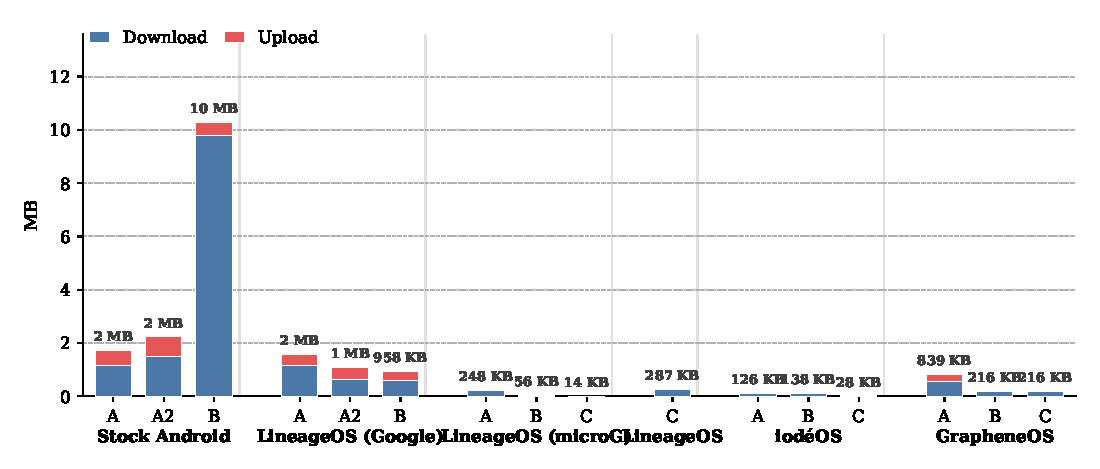
\includegraphics[width=\textwidth]{images/idle-data-usage.eps}
	\caption{Task 1: Idle data usage} \label{fig-idle-chart}
\end{figure}

Network activity observed during system idle following a reboot is presented in Figure \ref{fig-idle-chart}. Stock Android again shows the highest data usage, though Scenario B exhibits unexpectedly elevated traffic compared to both Scenario A2 and Scenario A. This anomaly stems from substantial background communication with www.gstatic.com, likely triggered by automatic updates or application background activity during the measurement time.

LineageOS in Scenario C similarly deviate from anticipated patterns, generating more idle traffic than its microG variant. LineageOS made connections to agnss.goog (Google Assisted GNSS) and www.gstatic.com. The agnss.goog endpoint was also observed in LineageOS (microG) during other measurement tasks, indicating that the entire LineageOS family retains this Google-dependent location mechanism. Other alternative distributions either replace this component with independent implementations or allow users to disable it entirely. GrapheneOS exhibits virtually identical idle traffic in Scenarios B and C, confirming that sandboxed Google Play Services remain dormant when not actively invoked.

\begin{figure}
	\includegraphics[width=\textwidth]{images/apps-data-usage.eps}
	\caption{Task 2: Basic apps interactions data usage} \label{fig-apps-chart}
\end{figure}

Figure~\ref{fig-apps-chart} shows network activity during basic app interactions that should not require Internet connectivity. Stock Android dominates with substantial data usage mostly by uncontrolled updates. All alternative distributions demonstrate dramatically lower traffic, with de-Googled configurations remaining effectively silent. Notably, whenever official Google Play Services were present and a Google account logged in at least a single request to Google infrastructure occurred.

\subsection{Domain distribution and Google dependencies}

\begin{figure}
	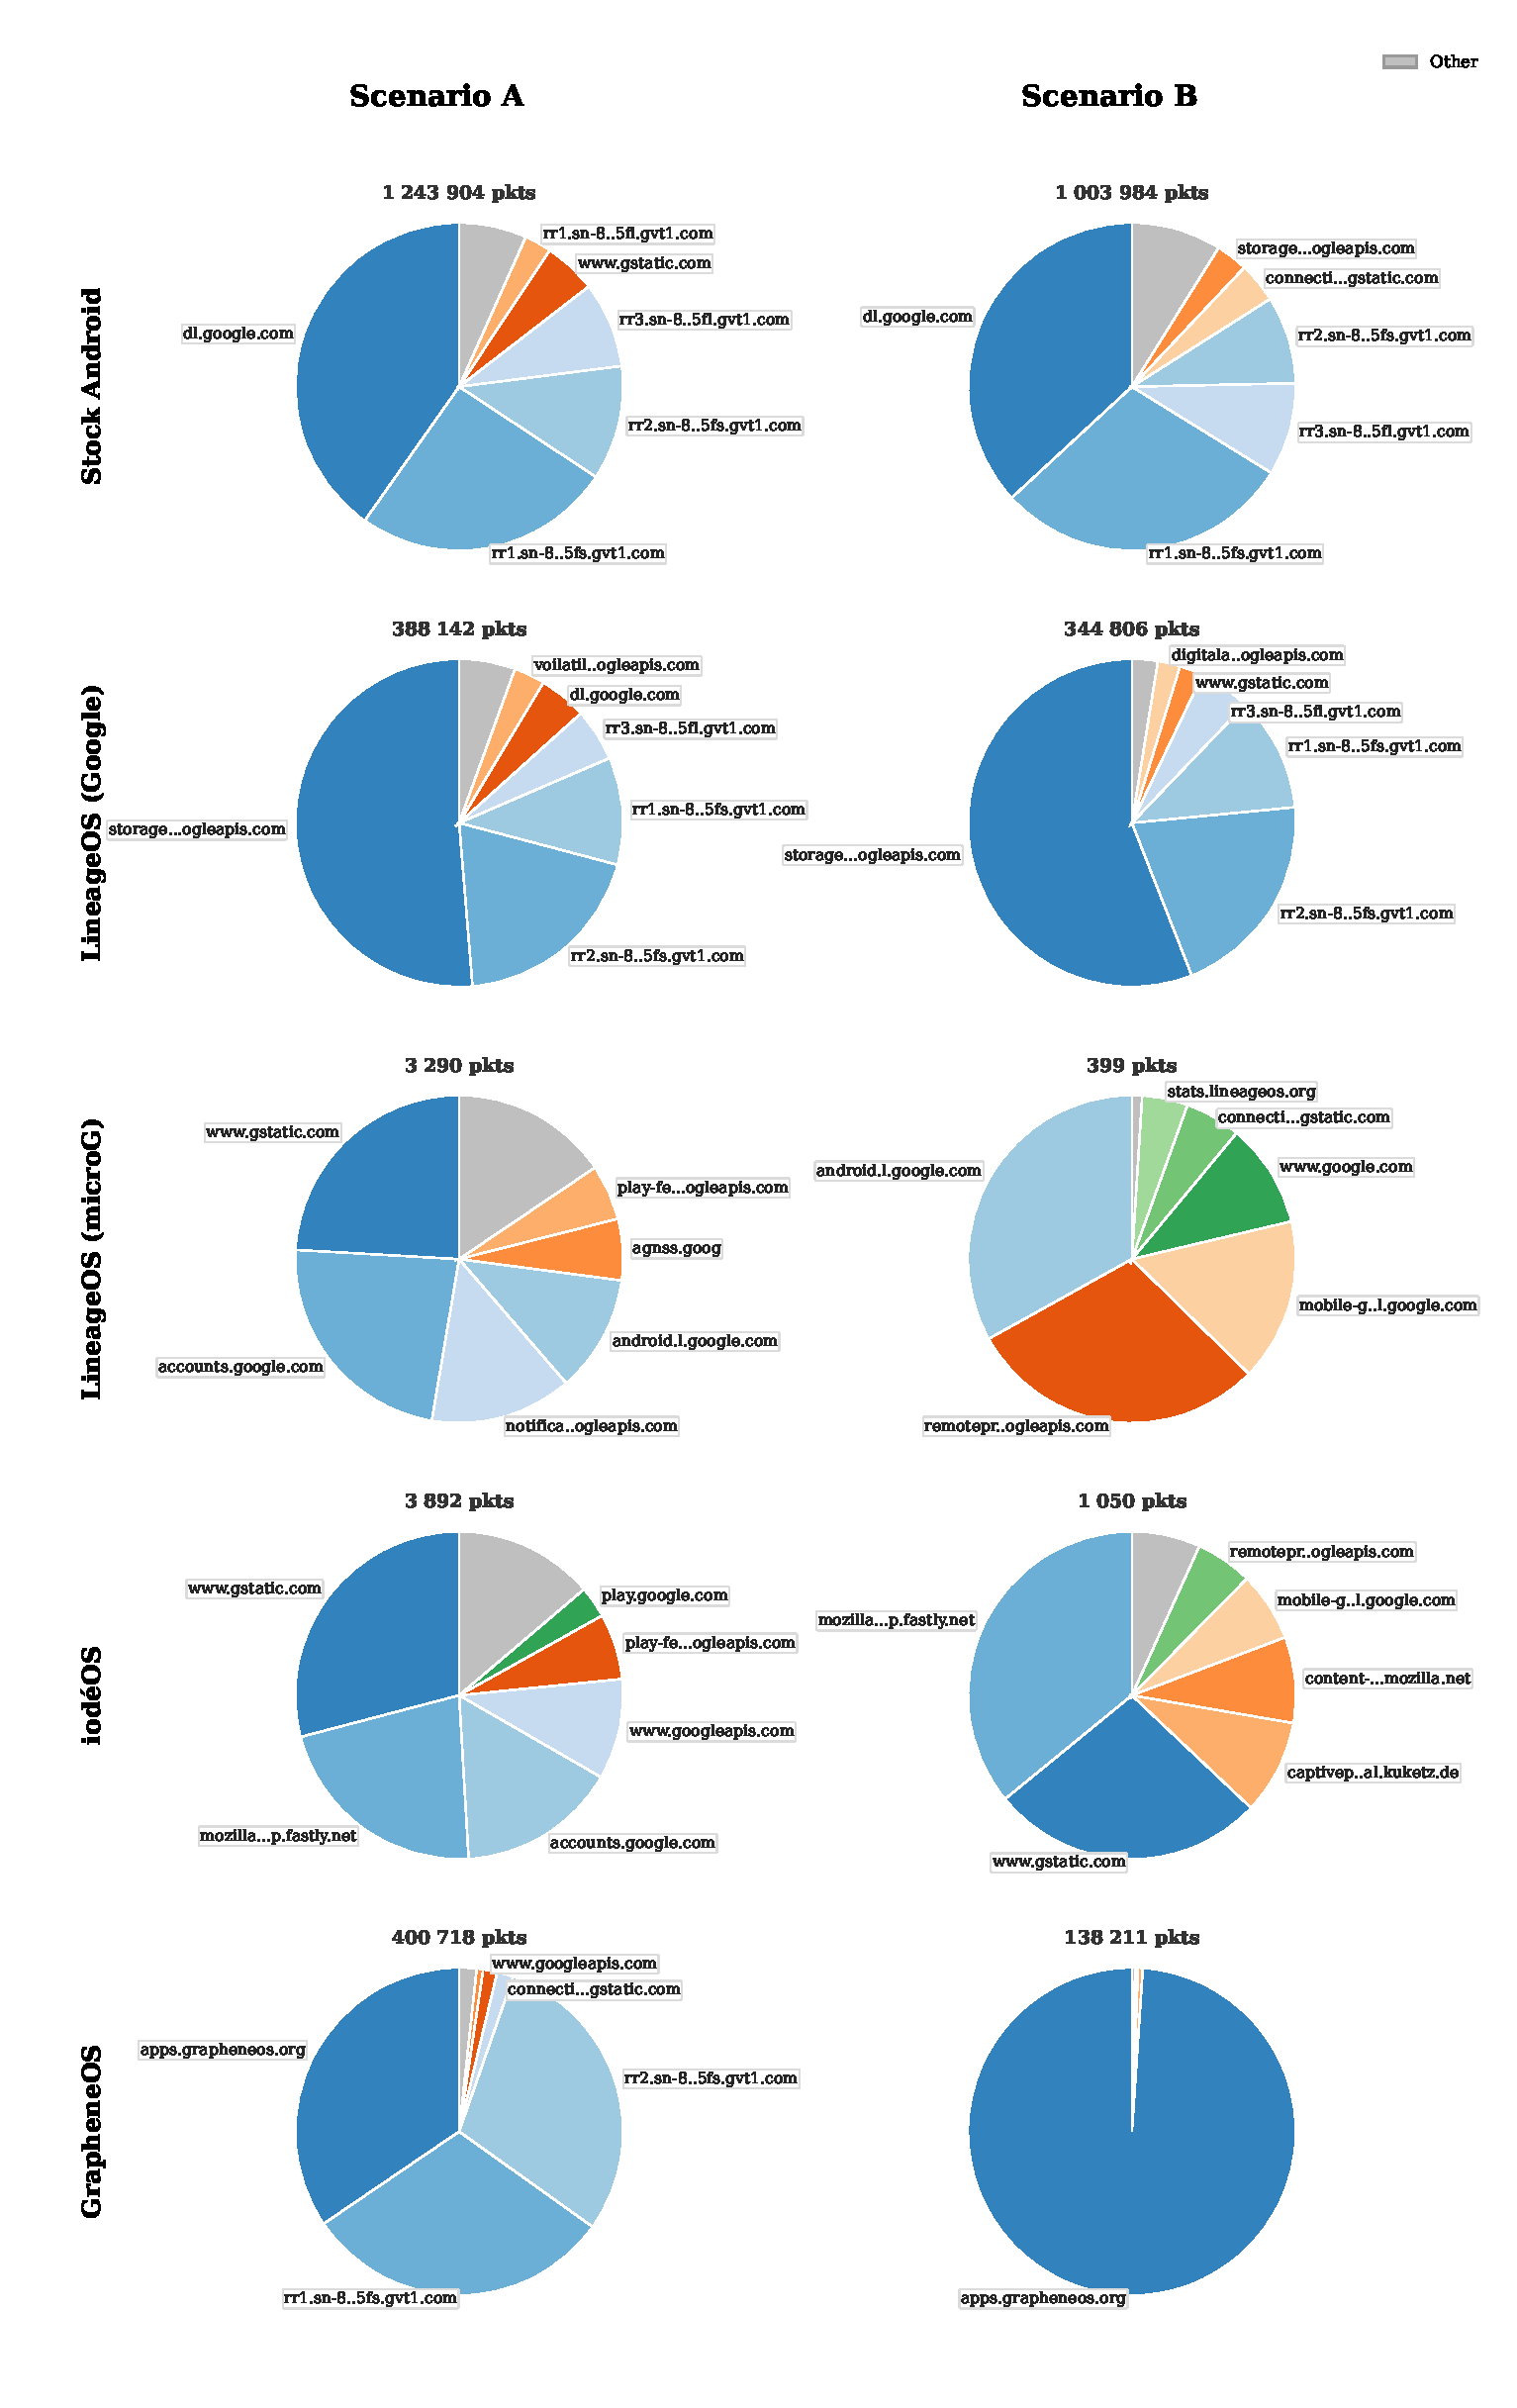
\includegraphics[width=\textwidth]{images/domains.eps}
	\caption{Domain-level distribution of network packets for scenarios A (with Google account) and B (without Google account, but Google Services present), aggregated over all tasks. Each pie shows the top domains by packet count for a given operating system and scenario.} \label{fig-domains-chart}
\end{figure}


[Lineageos uses SUPL from google, explain remoteprovisioning.googleapis.com, graphene makes no google connections by default, connectivity check is google on lineage]

[Table comparing google domains with replacements from other systems]